%-------------------------------------------------------------------------
% Design Project Input/Output Module Description
%-------------------------------------------------------------------------

\clearpage
\section{Current Input Module}
\label{sec-input-power}

This input module enables your IoT device to read the AC voltage and current
used to power lights, appliances, and everything else in your home. The emonTx
Shield you will use is an open-source energy monitoring and control
system suitable for domestic and industrial use. The emonTx will allow you to safely
measure the voltage and current that a lamp, for example, uses when plugged into
the wall.

You will be using an AC-to-AC adapter to measure voltage. Using a
transformer, the AC-to-AC adapter reduces the wall voltage down by a
factor of about 12, so \wu{110}{V} becomes \wu{9}{V}. If the wall
voltage changes, you will be able to see that change, reduced by a
factor of about 12. The current sensor is also a transformer. By
wrapping a ferrite loop around a wire, you can detect the induced
magnetic field from an AC current in the wire. This induced field
creates a voltage proportional to the current, which we can measure
using the Arduino. Power is current times voltage, or $P=IV$, so armed
with these two measurements we can calculate the power consumed by a
household device.

A sample circuit and Arduino code is shown below to get you started.
The emonTx plugs directly into the Arduino, the current sensors plug
into the \wu{3.5}{mm} audio jacks, and the AC-to-AC connector goes into
the barrel connector jack. We will share the voltage sensor across all
of the current sensors (note that current sensor 4 is disabled, so don't
use it). The sample code below will let you calculate power for the
devices connected to current sensor 1.

\vspace{0.1in}
\begin{minipage}[t]{0.49\tw}

  \vspace{0.0in}
  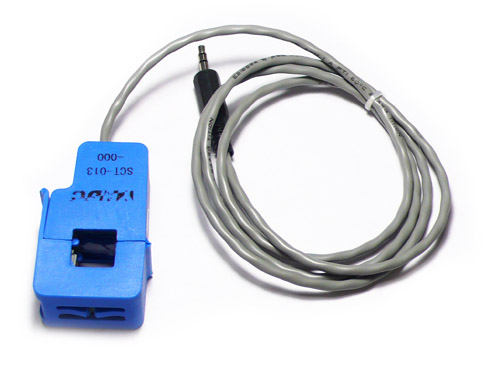
\includegraphics[width=\tw]{current-sensor.jpg}

  \vspace{0.0in}
  \begin{Verbatim}[gobble=3,fontsize=\small]
    #include "EmonLib.h"
    EnergyMonitor emon1;

    // Include an offset to "zero" the power
    float power_offset = 3.9;
  \end{Verbatim}

\end{minipage}
\hfill
\begin{minipage}[t]{0.49\tw}
  \vspace{0.1in}
  \begin{Verbatim}[gobble=3,fontsize=\small]
    void setup() {
      // Voltage: input pin, calibration, phase_shift
      emon1.voltage(0, 120.0, 1.7);

      // Current: input pin, calibration.
      emon1.current(1, 60.6);

      Serial.begin(9600);
    }

    void loop() {
      // Calculate all.
      // Params: num_half_wavelengths (crossings), time-out
      emon1.calcVI(20,2000);

      // Extract Real Power into variable
      float realPower = emon1.realPower - power_offset;

      // Extract Vrms into Variable
      float supplyVoltage = emon1.Vrms;

      // Floor the power at 0.
      if (realPower < 0.0)
        realPower = 0.0;

      Serial.print(realPower); Serial.print("W @ ");
      Serial.print(emon1.Vrms); Serial.println("V");
    }
  \end{Verbatim}
\end{minipage}

%Questions:
